
% \titlegraphic{\hfill\includegraphics[height=1.5cm]{logo.pdf}}

\documentclass[xcolor=pdftex,dvipsnames,table,numbers,hyperref={pdfpagelabels=false},compress]{beamer}
%\usepackage{requiredPackage}
\usepackage{amsmath}
\usepackage{graphicx}
\usepackage{amsfonts}
\usepackage{amssymb}

\usepackage{tabularx}
\usepackage{epstopdf}
\usepackage{overpic}
\usepackage{url}
\usepackage{calrsfs}
\usepackage{mathrsfs}
\usepackage{epsfig}
\usepackage{cancel}
\usepackage{changepage}

\usepackage{tikz}
\usepackage[customcolors]{hf-tikz} 

\usepackage{lmodern}
%\usepackage{mystyle}
\usepackage{subfig}
\usepackage{pifont}
\usepackage{tabu}
\usepackage{xcolor}
\usepackage{algorithm}
\usepackage{algpseudocode}
%\usepackage{enumitem}
\usepackage{remreset}
\usepackage{etoolbox}
\usepackage{comment} % end and begin comment
%\usepackage{dtklogos} 
\usepackage{listings}
\lstset{breaklines=true} 

\newcommand{\gline}{\textcolor{gray}{\hline}}
\newcommand{\cmark}{\ding{51}}%
\newcommand{\xmark}{\ding{55}}%
\newcommand{\gcheck}{\textcolor{blue}{\Large \cmark}}
\newcommand{\rcross}{\textcolor{red}{\Large \xmark}}
\newcommand{\tkt}{\tilde{K}_\theta}
\newcommand{\kt}{K_\theta}
\newcommand{\ind}{\overset{ind}{\sim}}
\newcommand{\plim}{\overset{p}{\rightarrow}}
\newcommand{\cx}{\frac {X'X}n}
\newcommand{\cz}{\frac {Z'Z}n}
\newcommand{\ccz}{\frac {Z'Z}n - \Sigma_A}
\newcommand{\czy}{\frac {Z'y}n}
\newcommand{\cyz}{\frac {y'Z}n}
\newcommand{\cxy}{\frac {X'y}n}
\newcommand{\cyx}{\frac {y'X}n}
\newcommand{\myitem}{\vskip3mm \item}

\newcommand{\calS}{{\cal S}}
\newcommand{\calA}{{\cal A}}
\newcommand{\calK}{{\cal K}}
\newcommand{\calX}{{\cal X}}
\newcommand{\calD}{{\cal D}}
\newcommand{\calG}{{\cal G}}
\newcommand{\calT}{{\cal T}}
\newcommand{\calU}{{\cal U}}
\newcommand{\calR}{{\cal R}}
\newcommand{\tp}{\tilde{p}}
\newcommand{\tildebC}{\tilde{\bC}}
\newcommand{\calL}{{\cal L}}

\newcommand{\blam}{ \mbox{\boldmath $ \lambda $} }
\newcommand{\bet}{ \mbox{\boldmath $ \eta $} }
\newcommand{\bome}{ \mbox{\boldmath $ \omega $} }
\newcommand{\bbet}{ \mbox{\boldmath $ \beta $} }
\newcommand{\bbeta}{ \mbox{\boldmath $ \beta $} }
\newcommand{\balph}{ \mbox{\boldmath $ \alpha $} }
\newcommand{\balpha}{ \mbox{\boldmath $ \alpha $} }
\newcommand{\bphi}{ \mbox{\boldmath $\phi$}}
\newcommand{\bzeta}{ \mbox{\boldmath $\zeta$}}
\newcommand{\bkap}{ \mbox{\boldmath $\kappa$}}
\newcommand{\bkappa}{ \mbox{\boldmath $\kappa$}}
\newcommand{\beps}{ \mbox{\boldmath $\epsilon$}}
\newcommand{\bepsilon}{ \mbox{\boldmath $\epsilon$}}
\newcommand{\bthet}{ \mbox{\boldmath $ \theta $} }
\newcommand{\btheta}{ \mbox{\boldmath $ \theta $} }
\newcommand{\blambda}{ \mbox{\boldmath $ \lambda $} }
\newcommand{\bnu}{ \mbox{\boldmath $\nu$} }
\newcommand{\bmu}{ \mbox{\boldmath $\mu$} }
\newcommand{\bGam}{ \mbox{\boldmath $\Gamma$} }
\newcommand{\bSig}{ \mbox{\boldmath $\Sigma$} }
\newcommand{\bSigma}{ \mbox{\boldmath $\Sigma$} }
\newcommand{\bPhi}{ \mbox{\boldmath $\Phi$} }
\newcommand{\bThet}{ \mbox{\boldmath $\Theta$} }
\newcommand{\bTheta}{ \mbox{\boldmath $\Theta$} }
\newcommand{\bDel}{ \mbox{\boldmath $\Delta$} }
\newcommand{\bDelta}{ \mbox{\boldmath $\Delta$} }
\newcommand{\bnabla}{ \mbox{\boldmath $\nabla$} }
\newcommand{\bLam}{ \mbox{\boldmath $\Lambda$} }
\newcommand{\bLambda}{ \mbox{\boldmath $\Lambda$} }
\newcommand{\bgam}{ \mbox{\boldmath $\gamma$} }
\newcommand{\bgamma}{ \mbox{\boldmath $\gamma$} }
\newcommand{\brho}{ \mbox{\boldmath $\rho$} }
\newcommand{\bdel}{ \mbox{\boldmath $\delta$} }
\newcommand{\bdelta}{ \mbox{\boldmath $\delta$} }
\newcommand{\sis}{\sigma^2}
\newcommand{\bOmega}{\mbox{\boldmath $\Omega$} }
\newcommand{\bPsi}{ {\boldsymbol \Psi} }
\newcommand{\btkt}{\boldsymbol{\tilde{K}}_\theta}
\newcommand{\pg}{P{\'o}lya-Gamma }

\newcommand{\bzero}{\textbf{0}}
\newcommand{\bones}{\textbf{1}}
\newcommand{\ba}{\textbf{a}}
\newcommand{\bb}{\textbf{b}}
\newcommand{\bB}{\textbf{B}}
%\newcommand{\bA}{\textbf{A}}
\newcommand{\bc}{\textbf{c}}
\newcommand{\bC}{\textbf{C}}
\newcommand{\bA}{\textbf{A}}
\newcommand{\bd}{\textbf{d}}
\newcommand{\bD}{\textbf{D}}
\newcommand{\be}{\textbf{e}}
\newcommand{\bE}{\textbf{E}}
\newcommand{\bk}{\textbf{k}}
\newcommand{\bK}{\textbf{K}}
\newcommand{\bh}{\textbf{h}}
\newcommand{\bs}{\textbf{s}}
\newcommand{\bS}{\textbf{S}}
\newcommand{\bH}{\textbf{H}}
\newcommand{\bI}{\textbf{I}}
\newcommand{\bt}{\textbf{t}}
\newcommand{\bu}{\textbf{u}}
\newcommand{\bv}{\textbf{v}}
\newcommand{\bw}{\textbf{w}}
\newcommand{\bW}{\textbf{W}}
\newcommand{\bx}{\textbf{x}}
\newcommand{\bX}{\textbf{X}}
\newcommand{\by}{\textbf{y}}
\newcommand{\bY}{\textbf{Y}}
\newcommand{\bz}{\textbf{z}}
\newcommand{\bZ}{\textbf{Z}}
\newcommand{\bL}{\textbf{L}}
\newcommand{\br}{\textbf{r}}
\newcommand{\bR}{\textbf{R}}
\newcommand{\bm}{\textbf{m}}
\newcommand{\bM}{\textbf{M}}
\newcommand{\given}{\,|\,}
\newcommand{\T}{\top}
\newcommand{\bV}{\textbf{V}}
\newcommand{\bJ}{\textbf{J}}
\newcommand{\blue}[1]{{\color{RoyalBlue!90} #1}}
\newcommand{\red}[1]{{\color{Red} #1}}
\newcommand{\green}[1]{{\color{Green} #1}}
\newcommand{\orange}[1]{{\color{Orange} #1}}
\newcommand{\titl}[1]{{\begin{large}\begin{center}#1\end{center}\end{large}}}

\newcommand{\tildea}{\tilde{a}}
\newcommand{\tildeba}{\tilde{\ba}}
\newcommand{\tildebv}{\tilde{\bv}}
\newcommand{\tildev}{\tilde{v}}
\newcommand{\tildeA}{\tilde{A}}
\newcommand{\tildeC}{\tilde{C}}
\newcommand{\tildeK}{\tilde{K}}
\newcommand{\tildew}{\tilde{w}}
\newcommand{\tildeu}{\tilde{u}}
\newcommand{\tildebw}{\tilde{\bw}}
\newcommand{\tildeeps}{\tilde{\epsilon}}
\newcommand{\tildebeps}{\tilde{\bepsilon}}
\newcommand{\eps}{\epsilon}
\newcommand{\sigs}{\sigma^2}
\newcommand{\taus}{\tau^2}
\newcommand{\iid}{\stackrel{\mathrm{iid}}{\sim}}

%\newcommand{\calS}{{\cal S}}
\newcommand{\calC}{{\cal C}}

%\documentclass[10pt]{beamer}

\usetheme{metropolis}
\usepackage{appendixnumberbeamer}

\usepackage{booktabs}
\usepackage[scale=2]{ccicons}

\usepackage{pgfplots}
\usepgfplotslibrary{dateplot}

\usepackage{xspace}
\newcommand{\themename}{\textbf{\textsc{metropolis}}\xspace}

\makeatletter
\@addtoreset{subfigure}{framenumber}% subfigure counter resets every frame
\makeatother

\makeatletter
\@addtoreset{figure}{framenumber}% subfigure counter resets every frame
\makeatother

\setbeamertemplate{caption}{\raggedright\insertcaption\par}
\captionsetup[subfigure]{labelformat=empty}


\title[]{Hierarchical Modeling for Large Univariate Areal Data}
\author{Andrew Finley$^1$ \& Jeffrey Doser$^2$}
	
\institute{
\begin{tiny}$^1$Department of Forestry, Michigan State University.\\
$^2$Department of Integrative Biology, Michigan State University.\end{tiny}
}

\date{May 15, 2023}


\begin{document}

\maketitle

\begin{frame}{Areal data}
	\begin{figure}[t!]
		\centering
		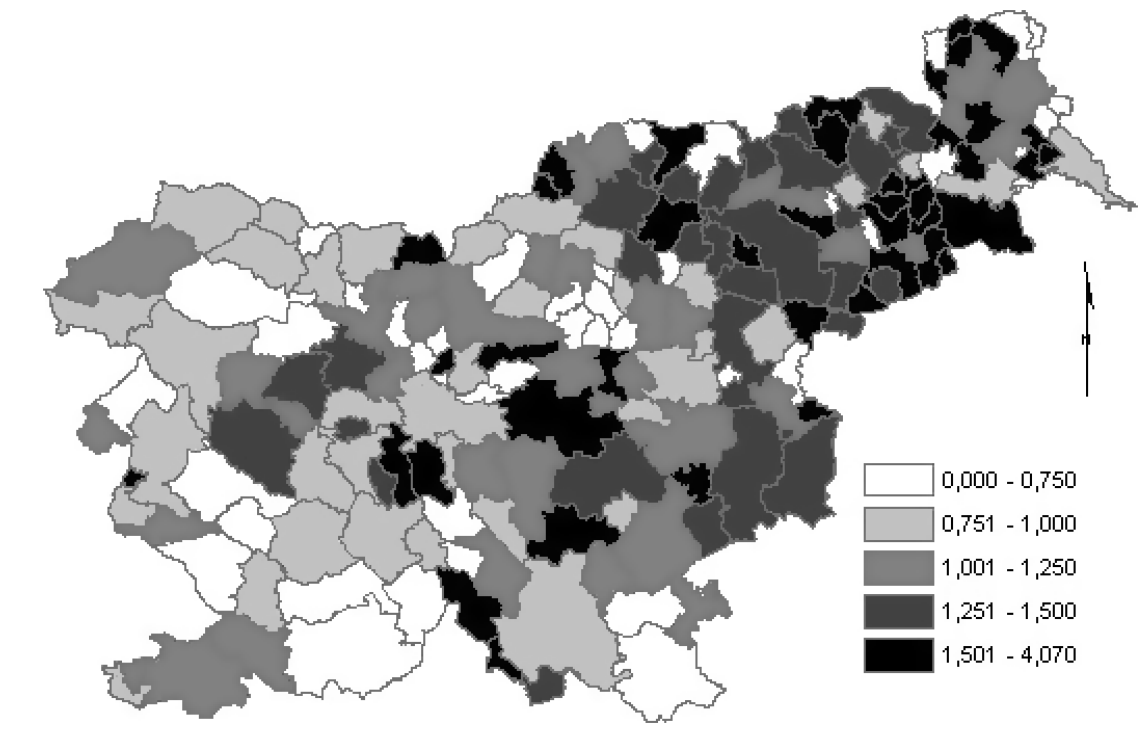
\includegraphics[scale=0.25]{../figures/sloveniaOE.png}
		%	\subfloat[Socio-economic score]{
		%		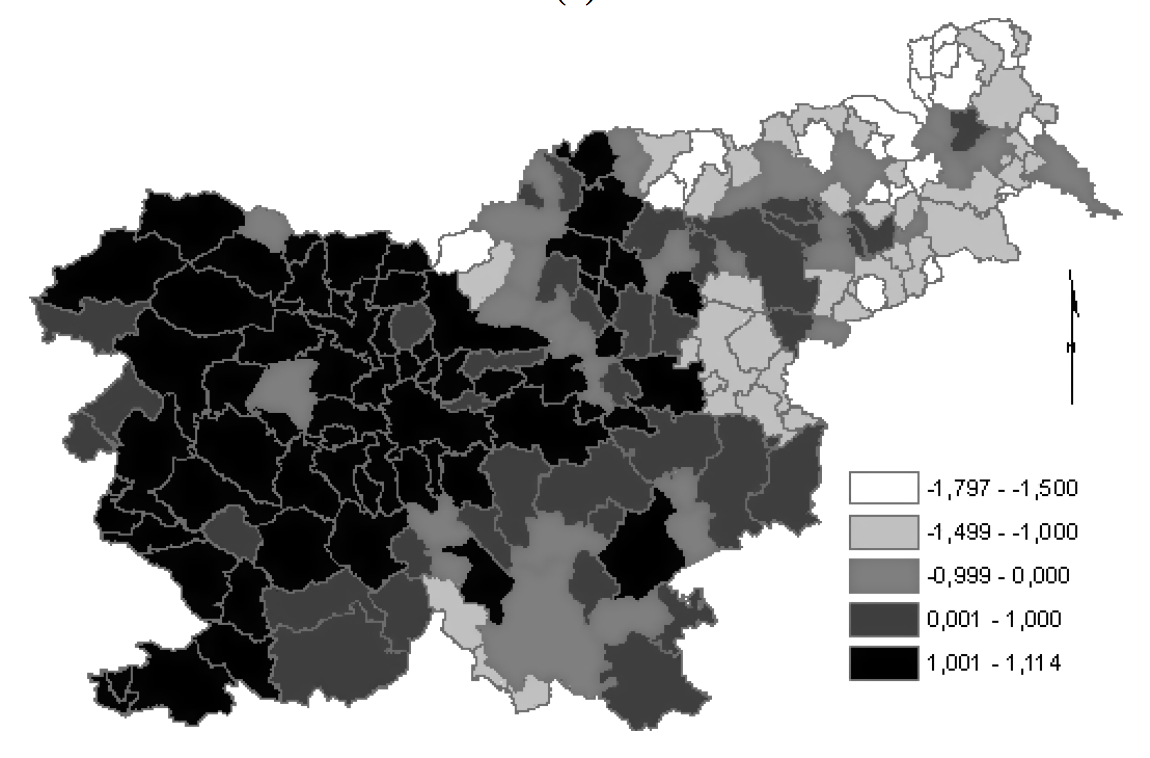
\includegraphics[scale=0.24]{../figures/sloveniaSIR.png}}
		\caption{Standardized stomach cancer incidence in 194 municipalities in Slovenia}
	\end{figure}
	\begin{itemize}
		\item Each datapoint is associated with a region like state, county, municipality etc.
		\item Usually a result of aggregating point level data
		%\item The spatial information is represented in terms of a graph depicting the relative orientation of the regions
	\end{itemize}
\end{frame}	

%\begin{frame}{Areal data}
%\begin{itemize}
%	\item Areal data
%	\begin{itemize}
%		\item Each observation is associated with a region like state, county etc.
%		\item Usually a result of aggregating point level data
%		\item The spatial information is represented in terms of a graph depicting the relative orientation of the regions
%\end{itemize}\end{itemize}
%\begin{figure}
%	\begin{center}
%		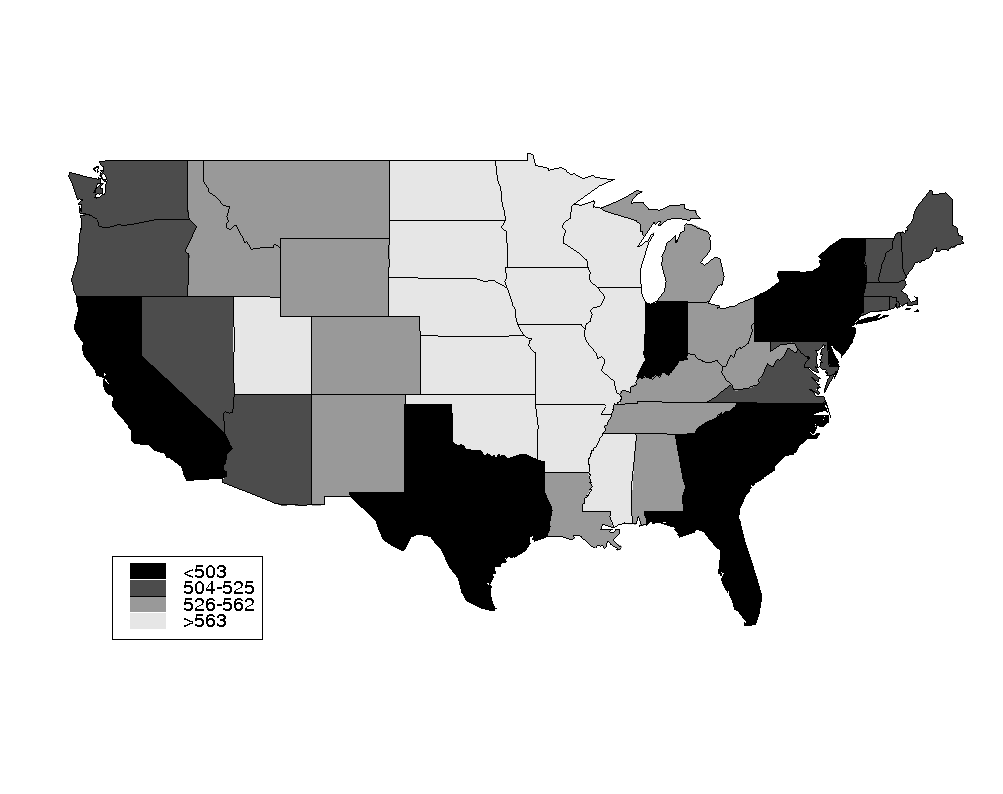
\includegraphics[scale=0.25,trim={1cm 4cm 1cm 4cm},clip] {figures/satmap.png}
%		\caption{SAT scores across the 48 contiguous states in the US}
%	\end{center}
%\end{figure}
%\end{frame}

\begin{frame}{Spatial disease mapping}
	\begin{figure}[t!]
		\centering
		\subfloat[Standardized cancer incidence]{
			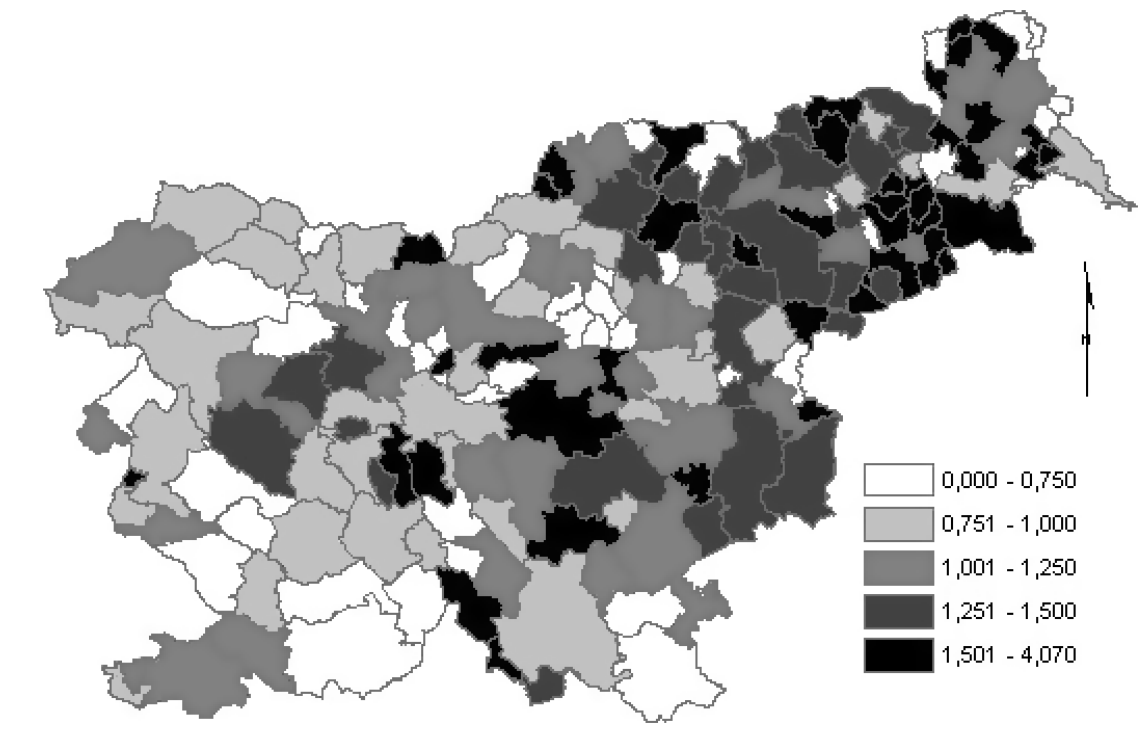
\includegraphics[scale=0.25]{../figures/sloveniaOE.png}}
		\subfloat[Socio-economic score]{
			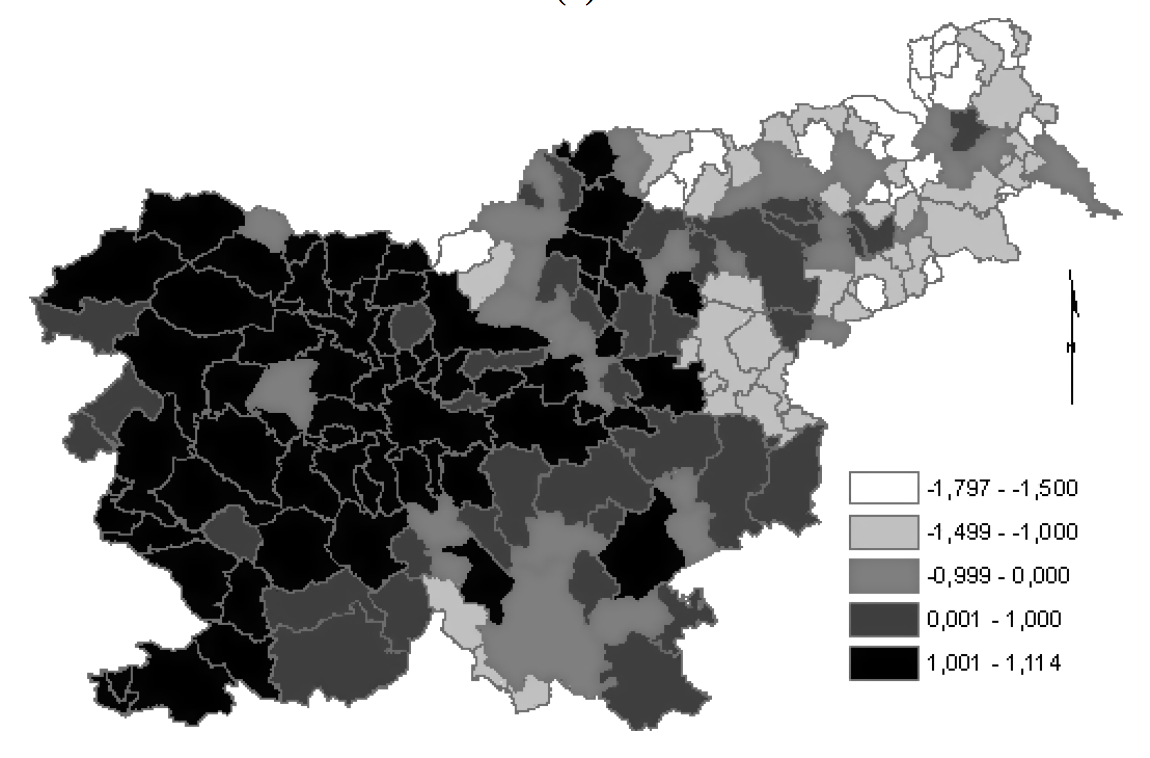
\includegraphics[scale=0.24]{../figures/sloveniaSIR.png}}
		\caption{Slovenia stomach cancer data}
	\end{figure}
	\begin{itemize}
		\item Goal: Identify factors (covariates) associated with the disease
		\item Goal: Identify \blue{spatial pattern}, if any, and smooth spatially
		\item Inference is often restricted only to the given set of regions 
	\end{itemize}
\end{frame}

\begin{frame}{GLM for Spatial disease mapping}
	\begin{itemize}
		\item At unit (region) $i$, we observe response $y_i$ and  covariate $x_i$
		\item $g(E(y_i)) = x'_i\beta + w_i $ where $g(\cdot)$ denotes a suitable link function
		\metroset{block=fill}
		\begin{alertblock}
		{Hierarchical areal model:}
		\[
		\prod_{i=1}^k p_1(y_i|x_i'\beta+w_i) \times N^{-1}(w \given 0, \tau_w Q(\rho)) \times p_2(\beta,\tau_w, \rho)
		\]
		\end{alertblock}
		\item \green{Notation:} $N^{-1}(m,Q)$ denotes normal distribution with mean $m$ and \alert{precision} (\red{inverse} covariance) $Q$
		\item $p_1$ denotes the functional form of the density corresponding to the link $g(\cdot)$
		%\item $Q(\rho)$ denotes the precision matrix corresponding to the model used 
	\end{itemize}
\end{frame}

\begin{frame}{How to model $Q(\rho)$}
	\begin{itemize}
		\item Choice of $Q(\rho)$ should enable spatial smoothing
		\myitem One possibility: Represent each region by a single point and use Gaussian Process covariance i.e. $Q(\rho)^{-1}_{ij} = C(m(i),m(j))$
		\myitem Many possible choices to map the region $i$ into a Euclidean coordinate $m(i)$
		\myitem Is it appropriate to represent a large area with a single point?
		\myitem Also GP approach is computationally very \red{expensive}
		\myitem \green{Alternate approach:} Represent spatial information in terms of a graph depicting the relative orientation of the regions
	\end{itemize}
\end{frame}

\begin{frame}{CAR models}
	\begin{itemize}
		\item \alert{Conditional autoregressive (CAR)} model (Besag, 1974; Clayton and Bernardinelli, 1992)
		\item Areal data modeled as a graph or network: $V$ is the set of vertices (regions)
		\item \blue{$i \sim j$} if regions $i$ and $j$ share a common border
		\item \alert{Adjacency matrix $A=(a_{ij})$} such that $a_{ij}= I(i \sim j)$
		\item $n_i$ is the number of neighbors of $i$
		\item CAR model:
		\begin{equation*}
		w_i \given w_{-i} \sim N^{-1}(\frac \rho{n_i}\sum_{j \given i \sim j} w_j, \tau_w n_i)
		\end{equation*}
	\end{itemize}
\end{frame}

\begin{frame}{CAR models}
	\begin{itemize}
		\item CAR model:
		\begin{equation*}
		w_i \given w_{-i} \sim N^{-1}(\frac 1{n_i}\sum_{j \given i \sim j} w_j, \tau_w n_i)
		\end{equation*}
		\myitem $w=(w_1,w_2,\ldots,w_k)' \sim N^{-1}(0, \tau_w (D-\rho A))$ where $D=diag(n_1,n_2,\ldots,n_k)$
		\only<1-2>{\myitem $\rho =1 \Rightarrow$ \red{Improper} distribution as $(D-A)1 = 0$ \alert{(ICAR)}
		\begin{itemize}
		\item Can be still used as a prior for random effects
		\item Cannot be used directly as a data generating model
		\end{itemize}}
		\only<2>{\myitem $\rho <1 \Rightarrow$ \red{Proper} distribution with added parameter flexibility}		
		%\myitem Often oversmooth spatial random effects
	\end{itemize}
\end{frame}

%\begin{frame}{Proper CAR model}
%	\vskip-7mm\begin{equation*}
%	w_i \given w_{-i} \sim N^{-1}(\frac \rho{n_i}\sum_{j \given i \sim j} w_j, \tau_w n_i)
%	\end{equation*}
%	\begin{itemize}
%		\item $w=(w_1,w_2,\ldots,w_k)' \sim N^{-1}(0, \tau_w (D-\rho A))$
%		%\item Proper probability distribution
%		\item \blue {Advantages:}
%		\begin{itemize}
%			\item makes distribution proper
%			\item adds parametric flexibility
%			\item $\rho=0$ interpretable as independence
%		\end{itemize}
%		\item \red {Disadvantages:}
%		\begin{itemize}
%			%\item why should we expect $y_{i}$ to be a proportion of average of neighbors - sensible spatial interpretation?
%			\item calibration of $\rho$ as a correlation, e.g., (as reported in Banerjee et al. 2014)
%			\begin{align*}
%			\rho & = 0.80  \text{ yields }  0.1 \le \mbox{Moran's }I \le 0.15,\\
%			\rho & = 0.90  \text{ yields }  0.2 \le \mbox{Moran's }I \le 0.25,\\
%			\rho & = 0.99 \text{ yields } \mbox{Moran's }I \le 0.5
%			\end{align*}
%			\item So, used with random effects, scope of spatial pattern may be limited
%		\end{itemize}
%	\end{itemize}
%	
%\end{frame}

\begin{frame}{SAR models}
	\begin{itemize}
		\item \alert{Simultaneous Autoregressive (SAR)} model (Whittle, 1954)
		\item  Instead of taking the conditional route, SAR model proceeds by simultaneously modeling the random effects
		\[
		w_i =\rho \sum_{i \neq j} b_{ij} w_j + \eps_i \mbox{ for } i=1,2,\ldots,k
		\]
		\item $\eps_i \ind N^{-1}(0,\tau_i)$ are errors independent of $w$   
		\item A common choice is to define $b_{ij}=I(i \sim j) / n_i$
		\item  \blue{Joint distribution:} $w \sim N^{-1}(0,(I-\rho B)'F(I-\rho B))$, $B=(b_{ij})$ and $F=diag(\tau_1,\tau_2,\ldots,\tau_k)$ 
		\item $\rho =1 \Rightarrow$ \red{Improper} distribution
	\end{itemize}
\end{frame}

%\begin{frame}{SAR models}
%	\begin{itemize}
%		\myitem $w \sim N^{-1}(0,(I-B)'F(I-B))$ is once again an \red{improper} distribution
%		\myitem \blue{Proper SAR model}: $b_{ij}$ is defined as $\rho I(i \sim j) / n_i$. 
%		\myitem $w \sim N^{-1}(0,(I-\rho B)'F(I- \rho B))$
%		\myitem $I-\rho B$ is non-singular
%		\myitem Difficult to interpret $\rho$ (like the proper CAR model)
%	\end{itemize}
%\end{frame}

\begin{frame}{Interpretation of $\rho$ in proper CAR and SAR models}
	\begin{itemize}
	\only<1>{
				\item Calibration of $\rho$ as a correlation, e.g., (as reported in Banerjee et al. 2014)
			\begin{align*}
			\rho & = 0.80  \text{ yields }  0.1 \le \mbox{Moran's }I \le 0.15,\\
			\rho & = 0.90  \text{ yields }  0.2 \le \mbox{Moran's }I \le 0.25,\\
			\rho & = 0.99 \text{ yields } \mbox{Moran's }I \le 0.5
			\end{align*}
			\item So, used with random effects, scope of spatial pattern may be \red{limited}
}
		\only<2>{\item  $\rho$ cannot be interpreted as correlation between neighboring $w_i$'s (Wall, 2004; Assuncao and Krainski, 2009) 
		\begin{figure}
			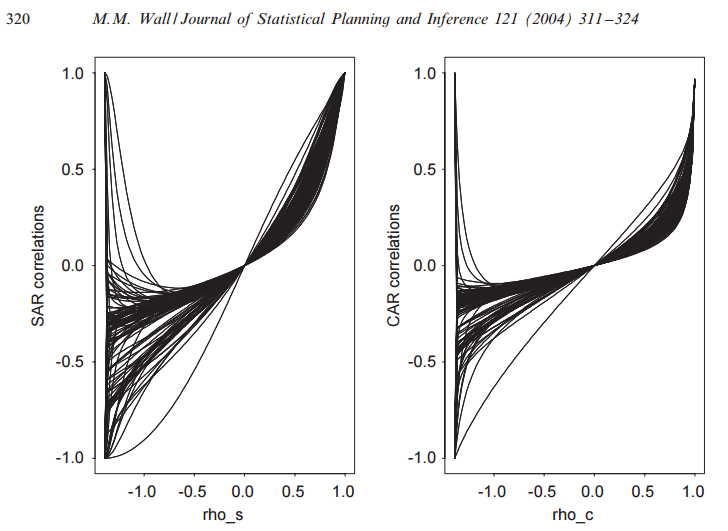
\includegraphics[scale=0.4]{../figures/wallcar.png}
		\caption{Neighbor pair correlations as a function of $\rho$ for proper CAR and SAR models over the graph of US states}
		\end{figure}}
		%\myitem $\det(D-\rho A)$ can be computationally intensive for large datasets
	\end{itemize}
\end{frame}

%\begin{frame}{Other areal models}
%	\begin{itemize}
%		\item Beyond the CAR and SAR models, the inventory of covariance models for areal datasets are very limited
%		\item Leroux et al. (2000) and MacNab and Dean (2000) extended the CAR model by accommodating over-dispersion alongside spatial information
%		\item  They proposed using the precision matrix $\lambda (D-A) + (1-\lambda) I$
%		\item $\lambda \in [0,1]$ controls the degree of dependence among the regions
%		\item Similar to proper CAR for regular graphs 
%		\item Computationally much more \red{expensive} than the proper CAR
%	\end{itemize}
%\end{frame}

\begin{frame}{SAR model and Cholesky factors}
	\begin{itemize}
		\item General SAR model: \[
		w_i = \sum_{i \neq j} b_{ij} w_j + \eps_i \mbox{ for } i=1,2,\ldots,k
		\]
		\item $w \sim N^{-1}(0, (I-B)'F(I-B))$ where $F=diag(\tau_1,\tau_2,\ldots,\tau_k)$
		\item Only \red{proper} when $I-B$ is \blue{invertible} which is not guaranteed for arbitrary $B$
		\item SAR is essentially modeling the precision matrix through the \blue{Cholesky} factor $I-B$
		\pause 
		\item Cholesky factors are not unique
		\item We can always choose a \blue{lower triangular} Cholesky factor
		%\item Similar approach to NNGP: $w_1 \sim N^{-1}(0,\tau_1)$, $w_i \given w_{\{j<i\}} \sim N^{-1}(\sum_{j <i} b_{ij} w_j, \tau_i)$
		%\myitem $w \sim N{-1}(0, (I-B)'F(I-B))$ where $F=diag(\tau_1,\tau_2,\ldots,\tau_k)$
		%\myitem Pros: For graphs neighbor sets are naturally chosen: $N(i) = \{ j \given j \sim i, j<i\}$
		%\myitem Cons: There is no joint distribution for $w$ from which we can obtain non-zero $a_{ij}$'s and $\tau_i$
		%\myitem Shortest distance matrix of graphs are not valid Euclidean distance matrices (EDM)
	\end{itemize}
\end{frame}

\begin{frame}{New model}
	\only<1>{\vskip-2mm\begin{align*}\label{eq:telescope}
	w_1 &= \eps_1 \nonumber \\
	w_2 &= b_{21} w_1 + \eps_2 \nonumber \\
	w_3 &= b_{31} w_1 + b_{32} w_2 + \eps_3 \\
	\vdots \nonumber \\
	w_k &= b_{k1} w_1 + b_{k1} w_2 + \ldots + b_{k,k-1} w_{k-1} + \eps_k \nonumber
	\end{align*}}
	\begin{itemize}
		\item \vskip-5mm \only<1>{ $B=(b_{ij})$ is now a strictly \red{lower triangular} matrix.}
		\only<2>{
		 \red{Advantages} of lower triangular $B$:
		\begin{itemize}
			\myitem $w \sim N^{-1}(0, (I-B)' F (I-B))$ is a \red{proper distribution} for any choice of lower triangular $B$
			\myitem $\det(L'FL)=\prod_{i=1}^n \tau_i$ where $F=diag(\tau_1,\ldots,\tau_k)$ and $L=I-B$
			\myitem $w'L'FLw=\tau_1w_1^2 \ + \sum_{i=2}^k \tau_i (w_i - \sum_{\{j < i\}} w_j b_{ij})^2$
			\myitem Likelihood $N^{-1}(w \given 0, (I-B)' F (I-B))$ can be computed using \red{$O(k+s)$ flops} where $s$ denotes the sparsity (number of non-zero entries) of $B$.
			\myitem Even if $k$ is large, evaluation of likelihood is fast if each region only shares border with a few others

		\end{itemize}}
	\end{itemize}
\end{frame}

\begin{frame}{Choice of $B$ and $F$}
	\begin{itemize}
		\item How to specify $B$ and $F$?
		\item Sparsity of $B$ is desirable
		\item If data had replicates for each region, there is large literature on fully data driven estimation of sparse Cholesky factors (Wu and Pourahmadi, 2003; Huang et al., 2006; Rothman
		et al., 2008; Levina et al., 2008; Wagaman and Levina, 2009; Lam and Fan, 2009)
		\item Unfortunately many areal datasets lack replication
	\end{itemize}
\end{frame}

\begin{frame}{Choice of $B$ and $F$}
	\begin{itemize}
		\item How to specify $B$ and $F$?
		\myitem Sparsity of $B$ is desirable
		\myitem Like in NNGP set $b_{ij}=0$ for $j$ outside neighbor sets $N(i)$
		%\item $F$ and the non zero $b_{ij}$'s are obtained from a Matern covariance function
		%\item Can we use this idea here for areal data?
%		\pause 
		\begin{itemize}
			\item \red{Pros:} For graphs neighbor sets are naturally chosen: $N(i) = \{ j \given j \sim i, j<i\}$
			\item \red{Cons:} There is no covariance function on arbitrary graphs from which we can obtain non-zero $b_{ij}$'s and $F$
		\end{itemize}
	\end{itemize}
\end{frame}

\begin{frame}{Autoregressive models on trees}
	\begin{itemize}
		%\item Shortest distance matrix of graphs are not valid Euclidean distance matrices (EDM)
\item $D=(d_{ij})$ is the shortest distance matrix on the graph
		\myitem If the graph was a tree (no loops), then $\rho^D = (\rho^{d_{ij}}$ is then a valid \alert{\em autoregressive} correlation matrix (AR(1) model on a tree, Basseville et al., 2006).
		\myitem Areal graphs are \red{loopy} and are not usually trees
\end{itemize}
\end{frame}

\begin{frame}{Local embedded spanning trees}
	\begin{itemize}
		%\item Recall $N(i)=\{j \given j\sim i, j <i\}$ and let $G_i$ subgraph of $G$
		\item \alert{Embedded spanning trees (EST)} of a graph $G$ is a subgraph of $G$ which is a tree and spans all the vertices of $G$
		\myitem Note that to specify $w_i = \sum_{j \in N(i)} b_{ij}w_j + \eps_i$ we only need a joint distribution on $\{i\} \cup N(i)$
		\myitem Let $G_i$ denote the subgraph of $G$ which includes vertices $\{i\} \cup N(i)$ and the edges among them
		\myitem The subgraph $T_i$ of $G_i$ which only contains the edges $\{ i \sim j \given j \in N(i)\}$ is an embedded spanning tree of $G_i$
		\myitem Use the \red{local} embedded spanning trees $T_i$ to specify the $b_{ij}$'s and $\tau_i$
		
	\end{itemize}
\end{frame}

\begin{frame}{Directed acyclic graph autoregressive (DAGAR) model}
	%\begin{itemize}
	%\item We specify $w_i \given w_{\{j<i\}} \sim N(\sum_{j \in N(i)} a_{ij} w_j, \tau_i)$ using a sequence of local s5panning trees
	%%\end{itemize}
	%\vskip -8mm\begin{figure}
	%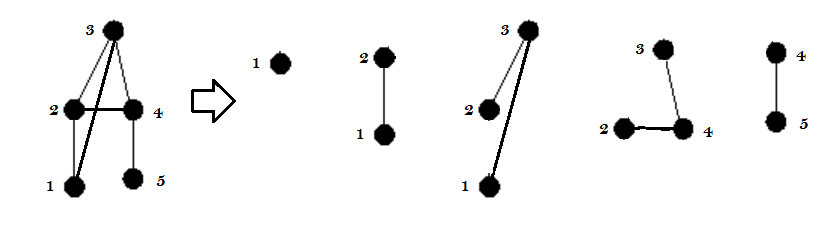
\includegraphics[scale=0.5]{../figures/dagar.png}
	%\end{figure}
	\begin{itemize}
		\vskip -10mm\item $AR_i$ denotes the $AR(1)$ distribution on $T_i$
		\item Solve for $b_{ij}$ and $\tau_i$ such that $E_{AR_i} (w_i \given w_{N(i)}) = \sum_{j \in N(i)} b_{ij} w_j $ and $\tau_i = 1/Var_{AR_i}(w_i \given w_{N(i)})$
		\item \red{No edge is left out !}
	\end{itemize}
\vskip -8mm		\begin{figure}
			\centering
			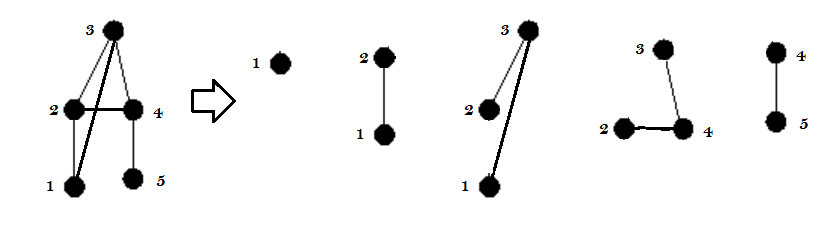
\includegraphics[scale=0.5]{../figures/dagar.png}
			\caption{Decomposing a graph into a sequence of embedded spanning trees}
		\end{figure}
\end{frame}

\begin{frame}{Properties of DAGAR models}
	\begin{itemize}
		\item  $b_{ij} = b_i = \rho/(1+(|N(i)|-1)\rho^2)$
		\myitem $\tau_i = (1+(|N(i)|-1)\rho^2)/(1-\rho^2)$
		\myitem $\det(Q_{DAGAR}) = \prod_{i=1}^k \tau_i$
		\myitem \red{Positive definite} for any $0 \leq \rho \leq 1$
		\myitem \red{Interpretability of $\rho$:} 
		\begin{itemize}
		\item If the graph is a tree, then \alert{DAGAR} model is same as the AR(1) model on the tree i.e. correlation between $d^{th}$ order neighbors is $\rho^d$ for $d=1,2,\ldots$
		\item If the graph is a closed two-dimensional grid, then each neighbor pair correlation is $\rho$
		\end{itemize}
		\myitem $p_{DAGAR}(w)$ can be stored and evaluated using \red{$O(e+k)$} flops where $e$ is the total number of neighbor pairs
	\end{itemize}
\end{frame}


\begin{frame}{Dependence on ordering}
	\begin{itemize}
		\item DAGAR model depends on the ordering of the regions when decomposing into local trees
		\myitem We can define a DAGAR model for every ordering 
		\myitem Spatial regions do not have natural ordering
		\myitem How to choose the ordering?
		\myitem Coordinate based orderings were used in Datta et al., 2016; Stein, 2004; Vecchia, 1988
		\myitem Model averaging over orderings ? Too many possibilities ($k!$)
	\end{itemize}
\end{frame}

\begin{frame}{Order-free model}
	\begin{itemize}
\only<1-2>{		\myitem Let $Q$ be the average over DAGAR precision matrices corresponding to all $k!$ possible orderings}
\only<2>{		\myitem $Q$ is \red{is free of ordering and available in closed form}
%	\end{itemize}
%	\metroset{block=fill}
%	\begin{alertblock}{Theorem} Let \alert{$i \approx j$} implies $i$ and $j$ share \blue{at least one common neighbor}. There exists functions $f(\rho,r)$ and $g(\rho,r)$ for any positive integer $r$ and $0 < \rho < 1$ such that: 
%		\begin{align*}
%		Q_{ii} &= 1 + \frac {n_i\rho^2}{2(1-\rho^2)} + \frac {\rho^2}{1-\rho^2} \sum_{j \sim i} f(\rho,n_j) \\
%		Q_{ij} &= -\frac{\rho}{1-\rho^2}I(i \sim j) + \frac {\rho^2}{1-\rho^2}I(i \approx j) \sum_{k \sim N(i) \cap N(j)} g(\rho,n_k)
%		\end{align*}
%	\end{alertblock}
%\end{frame}
%
%\begin{frame}{Order-free model}
%	\begin{itemize}
%		\item $Q$ is free of ordering
		\myitem $Q(i,j)$ is non-zero if and only if either $i \sim j$ or $i  \approx j$}
\only<3>{		\myitem Sparsity of $Q$ is $e_2$ where $e_2$ is the number of edges in the second order graph (\alert{moral graph}) created from $G$
		\myitem As $e_2 > e$, $Q$ is \blue{less sparse} than the CAR model or the ordered DAGAR model precision matrix and has higher flop count
		\myitem Total computational total cost for evaluating $Q$ is $O(e_2 n_{\max})$  
		\myitem $e_2 < kn_{\max}(n_{\max}+1)/2$ where $n_{\max} = \max (n_i)$ 
		\myitem If $n_{\max}$ is small, i.e., as long as each region only shares border with a few others (which is often the case), $Q$ is still quite \red{sparse} even for large $k$}
	\end{itemize}
\end{frame}

\begin{frame}{Interpretation of $\rho$}
	\vskip -1cm \begin{figure}
		\subfloat[path graph]{
			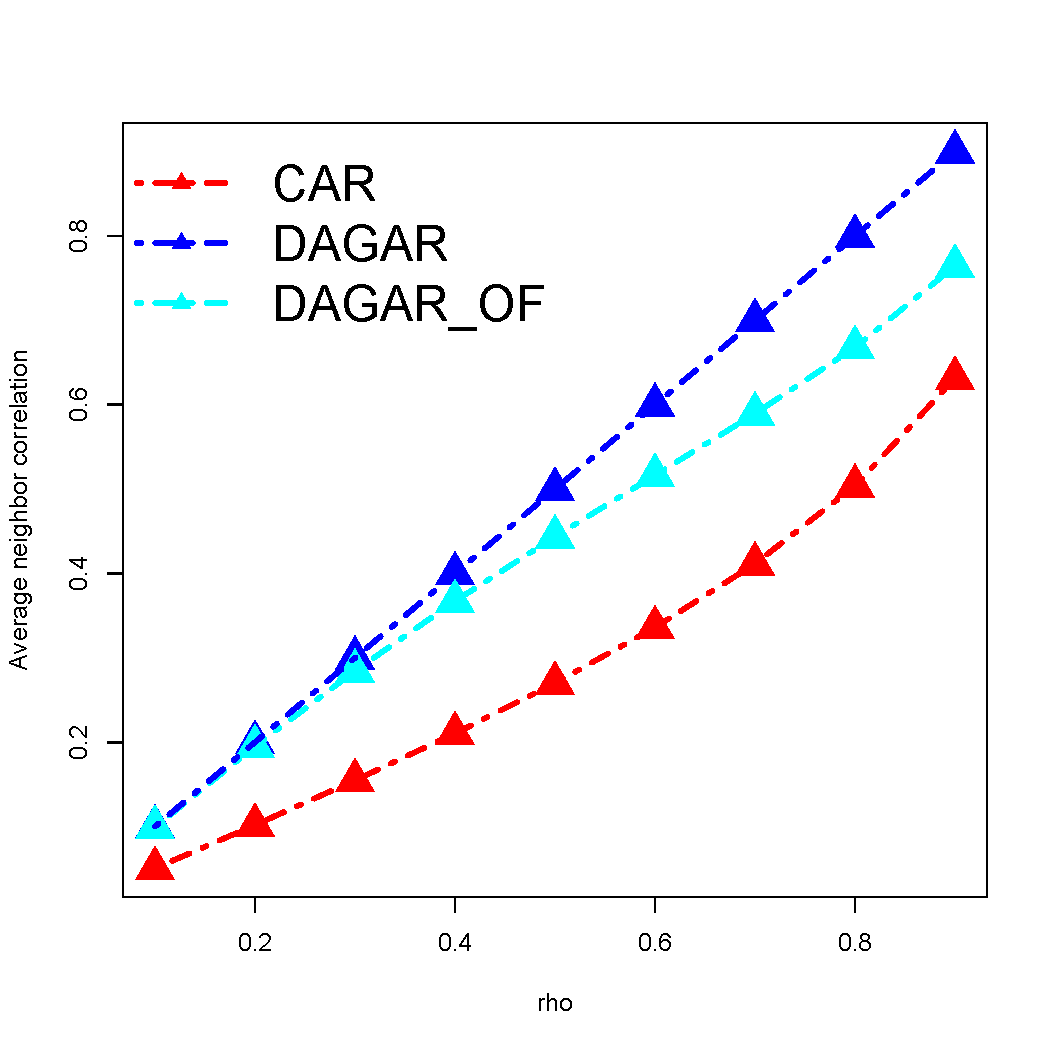
\includegraphics[scale=0.2]{../figures/rho_path.pdf}}
		\subfloat[grid graph]{
			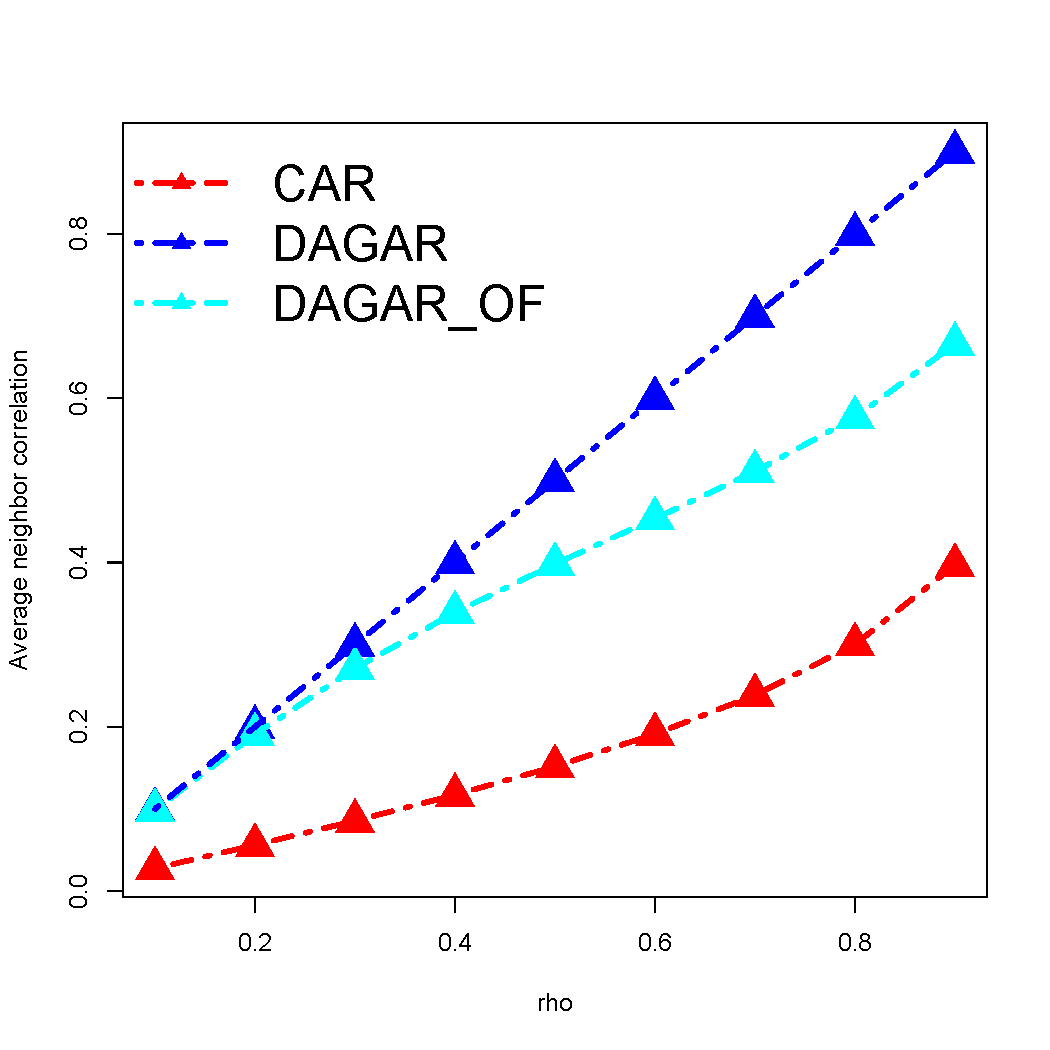
\includegraphics[scale=0.2]{../figures/rho_grid.pdf}}
		\subfloat[USA state map]{
			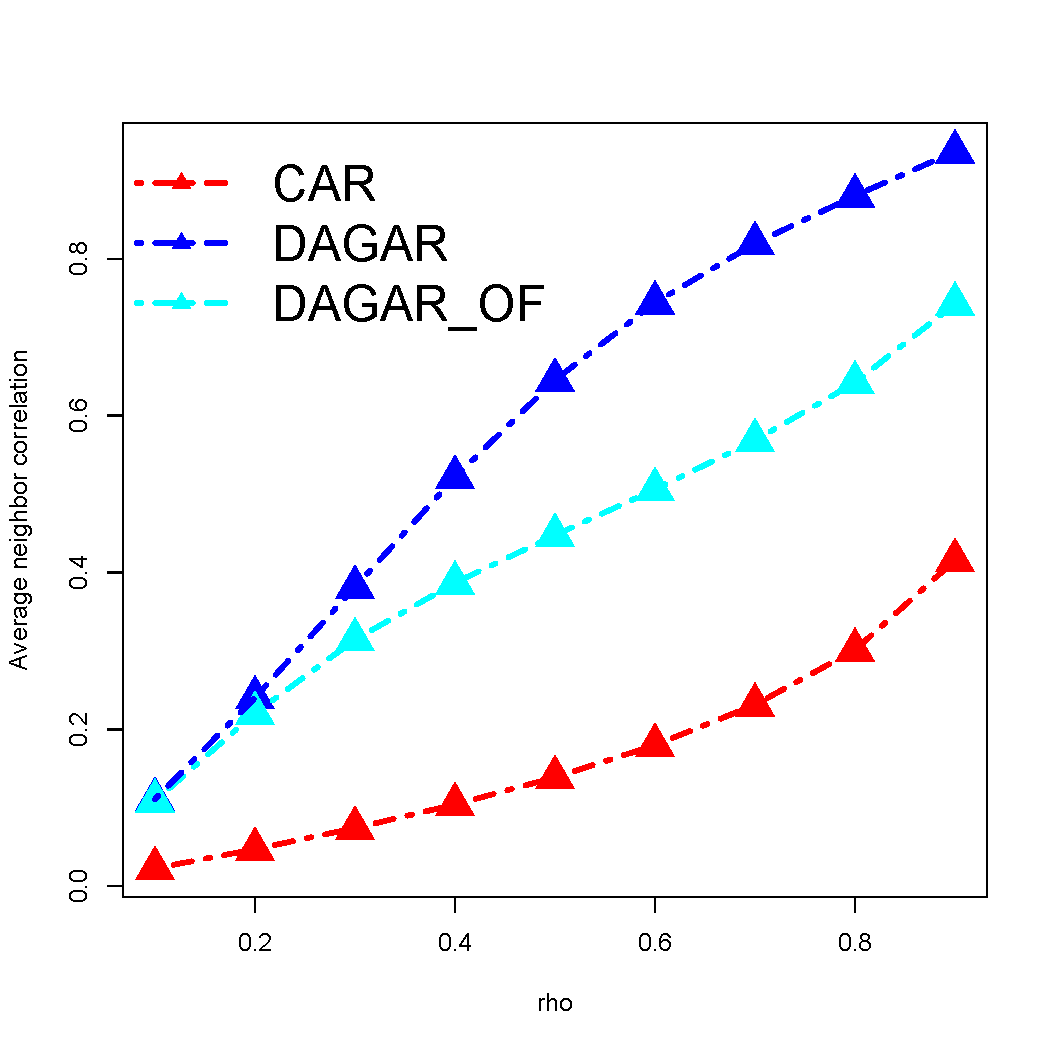
\includegraphics[scale=0.2]{../figures/rho_usa.pdf}}
			\caption{Average neighbor pair correlations as a funcion of $\rho$ for proper CAR and DAGAR models}
	\end{figure}
\end{frame}

\begin{frame}{Simulated data analysis}
	\vskip -4mm\begin{figure}
		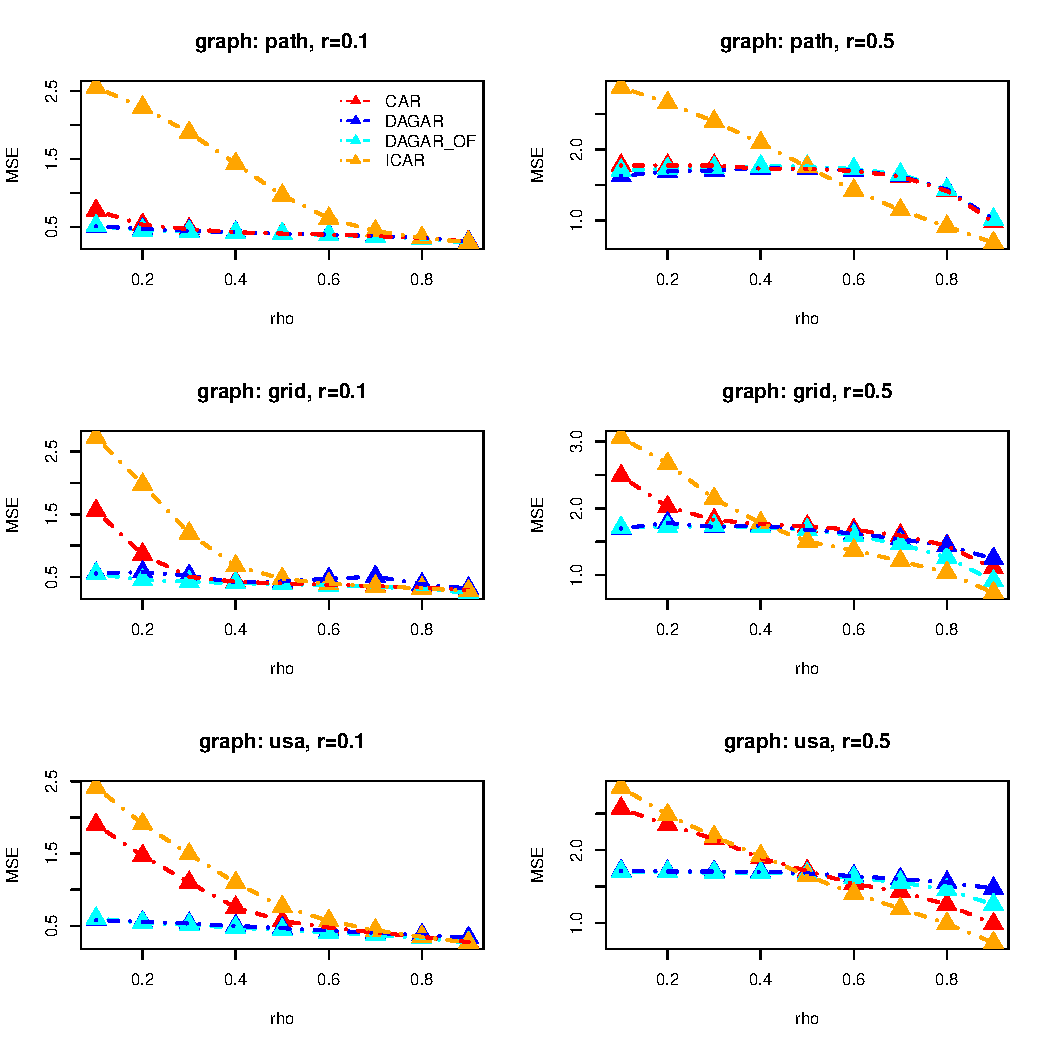
\includegraphics[scale=0.45]{../figures/mse.pdf}
		\vskip -6mm\caption{Mean square error as a function of $\rho$ and $r=\taus/\sigs$ for DAGAR and CAR models}
	\end{figure}
\end{frame}

\begin{frame}{Slovenia stomach cancer data}
	\begin{figure}[t!]
		\centering
		\subfloat[Standardized cancer incidence]{
			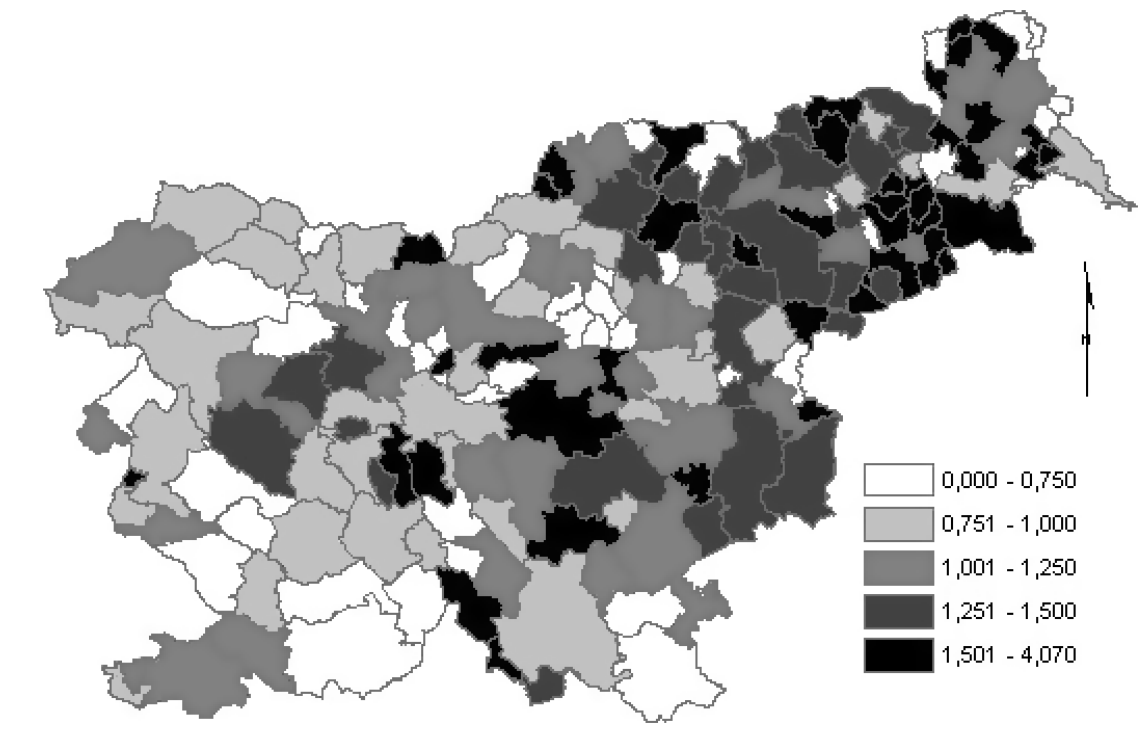
\includegraphics[scale=0.25]{../figures/sloveniaOE.png}}
		\subfloat[Socio-economic score]{
			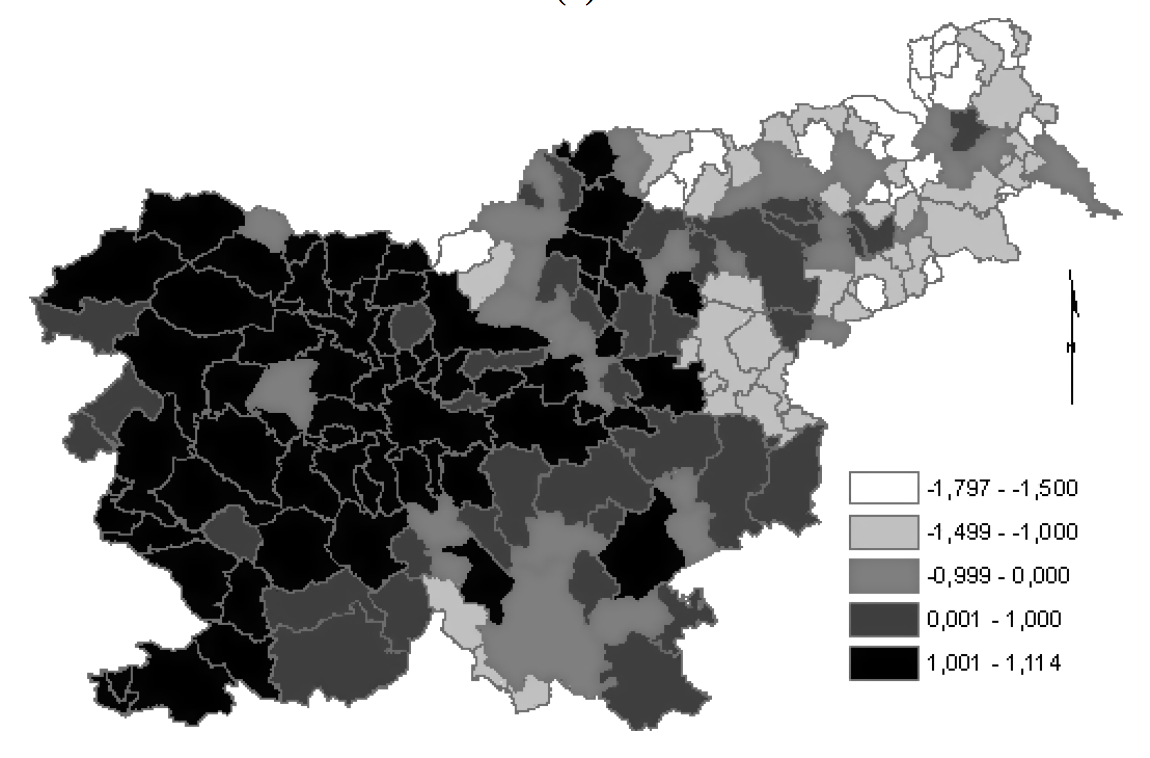
\includegraphics[scale=0.24]{../figures/sloveniaSIR.png}}
		\caption{Slovenia stomach cancer data}
	\end{figure}
	\begin{itemize}
		\item Observed ($O_i$) and expected ($E_i$) number of cancer counts for each of the $194$ municipalities of the country
		\item $O_i \sim Poisson(E_i \exp(\alpha+\beta SE_i + w_i))$ 
		where $w \sim N^{-1}(0,\tau_w Q(\rho))$
	\end{itemize}
\end{frame}

\begin{frame}{Slovenia stomach cancer data}
	\begin{table}[!h]
		\begin{tiny}
			\caption{Parameter estimates with confidence intervals and model comparison metrics}\label{tab:slov}
			\begin{tabular}{cccccc}
				& $\alpha$ & $\beta$ & $\rho$ & DIC & LPPD$_{LOOCV}$\footnote{Log-predictive posterior density using Leave one out cross validation} \\
				CAR & 0.09 (0.02, 0.16) & -0.12 (-0.19, -0.04) & 0.33 (0.02, 0.86) & 1097 & 1170 \\
				DAGAR & 0.11 (0.03, 0.18) & -0.12 (-0.19, -0.06) & 0.08 (0.004, 0.24) & 1091 & 1127 \\
				DAGAR$_{OF}$ & 0.11 (0.05, 0.17) & -0.12 (-0.18, -0.06) & 0.06 (0.003, 0.2) & 1090 & 1133 \\
			\end{tabular}
		\end{tiny}
	\end{table}
	\begin{itemize}
		\item Zadnik and Reich (2006) observed \alert{spatial confounding} with ICAR model ($\hat\beta_{ICAR} = -0.02 (-0.10, 0.06)$)
		\item Here for all three models the CIs for $\beta$ lie outside zero 
		%and the estimated coefficient of $\beta$ is negative
		\item Estimates of $\rho$ are much smaller than $1$
		\item Estimates of $\beta$ here are closer to those obtained in the non-spatial (NS) analysis $(\hat\beta_{NS} = -1.4 (-0.17, -0.10))$
	\end{itemize}
\end{frame}

\begin{frame}{Summary}
	\begin{itemize}
	    \item DAGAR models for areal data constructed from sparse Cholesky factors
	    \item \red{Scalability} for large areal data
		\item Ordered vs order-free DAGAR
		\begin{itemize}
			\item For all analysis, ordered model performed very similar to the order-free model
			\item Ordered model is faster with theoretical results about interpretability of $\rho$
%			\item \red{Advantages of ordered model:} 
%			\begin{itemize}
%				\item Massive scalability
%				\item Interpretability of $\rho$
%				\item Coherence
%				\item Possibility of doing asymptotics if networks are growing
%				\item Readily available Cholesky factorization will be very helpful for multivariate disease mapping
%			\end{itemize}
%			\item \red{Advantages of order-free model:} It is order free !
		\end{itemize}
		\item DAGAR models are \red{positive definite} and can be directly used to model or simulate any multivariate data on graphs (like imaging or social network data)
		\item Better performance than CAR modes for many scenarios
		\item DAGAR available at  https://arxiv.org/pdf/1704.07848.pdf
	\end{itemize}
\end{frame}

\end{document}
